\documentclass{sig-alternate-05-2015}
\usepackage{amsmath}
\usepackage{amssymb}
\DeclareMathOperator*{\argmax}{argmax}
\DeclareMathOperator*{\argmin}{argmin}

\usepackage{mathrsfs}

\begin{document}

\setcopyright{acmcopyright}

\title{Improving Collaborative Filtering with\\
Latent Time Model}

\numberofauthors{1}
\author{
\alignauthor
Chao Lv \quad
Lili Yao \quad
Yansong Feng \quad
Dongyan Zhao\titlenote{Corresponding author.}\\
\affaddr{Institute of Computer Science and Technology}\\
\affaddr{Peking University, Beijing 100871, China}\\
\email{\{lvchao, yaolili, fengyansong, zhaodongyan\}@pku.edu.cn}
}

\maketitle

\begin{abstract}
Collaborative filtering (CF) has been widely employed within
recommender systems in many real-world situations.
Its core idea is that items liked by the same user would be similar and
users like same items would share similar interest.
But it is not always true since users' interest changes as time goes on.
It should be more reasonable to say that
if two items are liked by the same user in the same time period,
there is a strong possibility that they are similar,
but the possibility will shrink if the user likes they in different time period.
In this paper,
we propose a latent time model to describe the time sensitive relationship
and integrate it into a feature based collaborative filtering framework
in order to improve the recommender performance.
The latent time model learns effective latent embeddings
for users and items in a neural network based language model.
Language model aims to extract the potential association
between sentences and words,
which is similar with users and items in recommender system.
The learned embedding for users and items can be considered as
a kind of latent side information because its dimension doesn't
have a actual meaning.
Experimental results on three MovieLens datasets demonstrate that
our approach can achieve the state-of-the-art performance.
\end{abstract}

\category{H.3.3}{Information Search and Retrieval}{Information Filtering}
\category{H.2.8}{Database Management}{Data Mining}
%\terms{Algorithms, Experimentation, Performance}
\keywords{Recommender System; Collaborative Filtering; Latent Side Information;}

\section{Introduction}
In the modern era of information overload,
recommender system has become more and more popular in many real-world situations.
Recommender system aims to help users find the items,
they are more likely to be interested in,
from huge amounts of candidates.
Lots of websites (e.g. Amazon, Netflix, Alibaba and Hulu) use recommender system to
target customers and provide them with useful information.
An excellent recommendation system can effectively increase the amount of sales.
For instance, 80\% of movies watched on Netflix
come from their recommender system \cite{gomez2015netflix}.

A widely used setting of recommender system is to
predict the rating a user will evaluate on a new item (such as a movie)
given the past rating history of the users.
Lots of classical recommendation methods have been proposed
during the last decade, and they can be categorized into two classes:
content based methods and collaborative filtering (CF) based methods.
Content based methods \cite{pazzani2007content} make use of
user profiles and item descriptions for recommendation.
CF based methods \cite{su2009survey} utilize
the past interactions or preferences, such as user ratings on items,
without using user or product content information.
CF based methods focus on predicting the preference of
one user by combining his feedback on a few items
and the feedback of all other users.
These methods have been developed for many years and
keep to be a hot area in both academia and industry
due to their impressive performance.

Among various CF based methods, matrix factorization (MF) based
collaborative filtering have become popular and
achieves the state-of-the-art performance \cite{koren2009matrix}.
Matrix factorization retrieves latent factors
from the sparse matrix of ratings.
Common latent factor techniques compute a low-rank rating matrix
by applying Singular Value Decomposition through gradient descent
\cite{koren2009matrix} or
Regularized Alternative Least Square algorithm \cite{zhou2008large}.
However, these methods are linear and cannot catch subtle factors.
Newer algorithms were explored to face those constraints such as
Non Linear Probabilistic Matrix Factorization \cite{pazzani2007content},
Factorization Machines \cite{rendle2010factorization} or
Local Low Rank Matrix Approximation \cite{lee2013local}.

Effective latent factors is the most important
core in matrix factorization based CF methods.
In recent years, deep learning \cite{hinton2006reducing, hinton2006fast}
has attracted a lot of attention due to its amazing performance
to learn representations on various tasks,
especially in computer vision and natural language processing.
However, neural networks have attracted little attention
in the collaborative filtering community.
With large-scale data and rich-side information available,
it is now practicable to learn latent factors
through deep learning.
Deep learning algorithms like Restricted Botzmann Machines (RBM)
\cite{salakhutdinov2007restricted},
Convolutional Neural Networks (CNN) \cite{wang2014improving} and
Stacked Denosing AutoEncoder (SDEA) \cite{wang2015collaborative}
are used directly for the task of collaborative filtering.

In this paper, we propose a latent time model and
integrate it into a feature based collaborative filtering framework.
Our latent time model takes advantage of the ratings time line
to address the problem that users' interest changes over time.
We first embed users and items into a low-dimensionality space,
and change the interest similarity over time into spacial distance.
In particular, we extract time sensitive interest distribution
of users and items via this embedding model.
Then, by leveraging a feature bases collaborative filtering framework,
it is quite natural to integrate the latent time model
into the whole prediction framework via side information pattern.
Latent time model can help describe the interest similarity of
users and items from an angle of time.

The main contributions of this paper include:
(1) we propose a latent time model to describe the interest
drifting for users on items over time and
use a neural network based language model to extract
time sensitive interest distribution of users and items.
(2) we treat time sensitive interest distribution of users and items
as a kind of side information, and integrate them into
a feature-based collaborative filtering framework.
(3) we perform a set of experiments on three public
MovieLens dataset to compare our proposed method
with the baseline systems.
And, the experimental results demonstrate that
our proposed approach can achieve the state-of-the-art performance.

The rest of the paper is organized as follows.
Section 2 gives an overview of the related work.
Then, we describe our latent time model in Section 3.
The experimental results as well as the comparisons with
the-state-of-arts are shown in Section 4.
Finally, we conclude the paper and
outline our future work in Section 5.

\section{Related Work}
In general, our work is closely related to matrix factorization,
and neural network. We will discuss them in the following subsections.

\subsection{Matrix Factoriztion}
Matrix factorization (MF) is the most popular collaborative filtering methods,
their success at the Netflix competition have demonstrated their strength,
and lots of variants of it have been proposed in specific settings.
\cite{koren2009matrix, bennett2007netflix}.
Basically, the given ratings matrix $\mathbf{R} \in \mathbb{R}^{N*M}$
consisting of the item preferences of the users can be decomposed as
a product of two low dimensional matrices $\mathbf{U} \in \mathbb{R}^{N*K}$
and $\mathbf{V} \in \mathbb{R}^{K*M}$.
$\mathbf{U}$ could be treated as a user-interest matrix while
$\mathbf{U}$ could be treated as a item-interest matrix.
$K$ is the amount of interest.
The decomposition can be carried out by a variety of methods
ranging from SVD based approaches \cite{mazumder2010spectral}
to the relatively new non-negative
matrix factorization approach \cite{lee2001algorithms}.

Another classical MF method is probabilistic matrix factorization
(PMF) \cite{salakhutdinov2011probabilistic}.
The underlying assumption behind this method is that
the prior probability distribution of the latent factors and
the probability of the observed ratings given the latent factors
follow a Gaussian distribution.
Many algorithms have been developed to enhance the performance of PMF,
by designing the Bayesian versions \cite{salakhutdinov2008bayesian, xu2013fast, shi2013scmf}.

However, matrix factorization methods suffer from the cold start problem,
i.e. what recommendations to make when a new user/item arrives in the system.
Another problem often presented in many real world applications is data sparsity.
Incorporating side information has shown promising performance
in collaborative filtering in such scenarios.

In genera, social recommendation and content recommendation
are two main kind of side information.
Social recommendation methods focus on using the social network
to improve rating estimation and item recommendation.
SoRec \cite{ma2008sorec} is proposed as a probabilistic matrix
factorization framework which incorporates trust network information
into user taste analysis.
Ma \textit{et al.} \cite{ma2011recommender} also propose a matrix factorization framework
with social regularization based on the assumption
that users’ interests should be similar to those of their friends.
Based on these works, Yang \textit{et al.} \cite{yang2011like}
devise a factorbased random walk model to explain friendship connections,
and simultaneously use a coupled latent factor model to uncover interest interactions.
Content recommendation methods aim at utilizing item content
to improve rating prediction and item recommendation.
Pazzani \textit{et al.} \cite{pazzani2007content}
proposed content based recommendation system
which uses $tf \times idf$ method to get item representation,
then average them to estimate user profile.
Wang \textit{et al.} \cite{wang2011collaborative}
proposed a Bayesian Matrix Factorization (BMF) approach
with Latent Dirichlet Allocation (LDA) to extract topic
information from item content.

\subsection{Nerual Network}
\subsubsection{Nerual Network based Collaborative Filtering}
Neural Networks have attracted little attention in the
collaborative filtering community.
Salakhutdinov \textit{et al.} \cite{salakhutdinov2007restricted} were the first
work to tackle the Netflix challenge using Restricted Boltzmann Machines (RBM).
They modified the RBM as a two-layer undirected graphical model
consisting of binary hidden units and softmax visible units,
and tested their model on the Netflix dataset and
showed a comparable result with the start-of-the-art.

On music recommendation, van \textit{et al.} \cite{van2013deep}
and wang \textit{et al.} \cite{wang2014improving}
directly use Convolutional Neural Network (CNN)
or Deep Belief Networks (DBN)
to assist representation learning for content information.
Sedhain \textit{et al.} \cite{sedhain2015autorec} and
Strub \textit{et al.} \cite{strub2015collaborative}
directly train Autoencoders to provide the best predicted ratings.
Those methods report excellent results in the general case.
However, the cold start problem is not solved.

Wang \textit{et al.} \cite{wang2015collaborative} 
directly coupled matrix factorization with deep learning models,
and proposed a hierarchical Bayesian model called
Collaborative Deep Learning (CDL)
which tightly couples Stacked Denoising AutoEncoders (SDA) and
Collaborative Topic Regression (CTR) to
solve the cold start problem.
Li \textit{et al.} \cite{li2015deep} proposed the
marginalized Stacked Denoising AutoEncoders (mSDA) which
is close to CDL but more efficient and scalable.
Meanwhile, their model can learn deep features for both items and users
while CDL only extracts deep features for items.

\subsubsection{Nerual Network based Language Model}
Traditional language model uses a one-hot representation
to represent each word as a feature vector,
where these feature vectors have the same length
as the size of vocabulary, and the position that
corresponds to the observed word is equal to 1, and 0 otherwise.
However, this approach often exhibits significant limitations in practical tasks,
suffering from high dimensionality and severe data sparsity.

Mikolov \textit{et al.} \cite{mikolov2013efficient, mikolov2013distributed}
proposed the word2vec algorithm to address these issues.
They take advantage of the word order in text documents,
explicitly modeling the assumption that closer words
in the word sequence are statistically more dependent.
The continuous bag-of-words (CBOW) and skip-gram (SG)
language models are highly scalable for learning word
representations from large-scale corpora.
Le \textit{et al.} \cite{le2014distributed} followed the above
work and proposed the paragraph2vec algorithm to simultaneously
learn vector representations of sentence and words
by considering the sentence as a ``global context".

\section{Our Approach}
In this section,
we first describe the definition of the task to be solved and
the notation we are going to use in this paper. 
Then we introduce our embedding model to extract the relationship
between users and items based on the local interest and global interest.
In the last, we utilize the embedding information as pseudo side information
in the machine learning model to do the final prediction.

\subsection{Problem Definition}
Given $N$ users and $M$ items, the rating $r_{ij}$ is the rating given by
the $i^{th}$ user for the $j^{th}$ item.
In the common real-world situations,
users usually rate on a fraction of items, not on the whole items.
Therefore,
those ratings entail a sparse matrix $\mathbf{R} \in \mathbb{R}^{N \times M}$,
as illustrated in Figure \ref{fig:matrix}.
The goal of recommender system is to make a prediction on the missing ratings.
Based on that, we will know the preference of a user on the items he never rates,
and recommend high score items to him.

\begin{figure}[htbp]
	\centering
	% 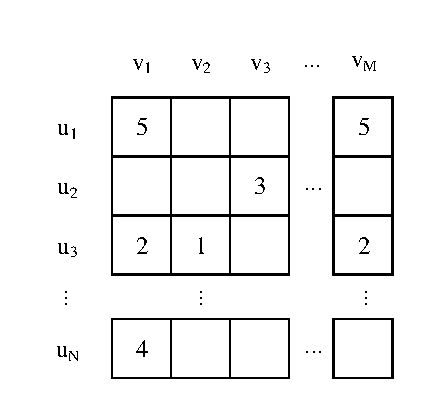
\includegraphics[scale=0.8]{images/3.pdf}
	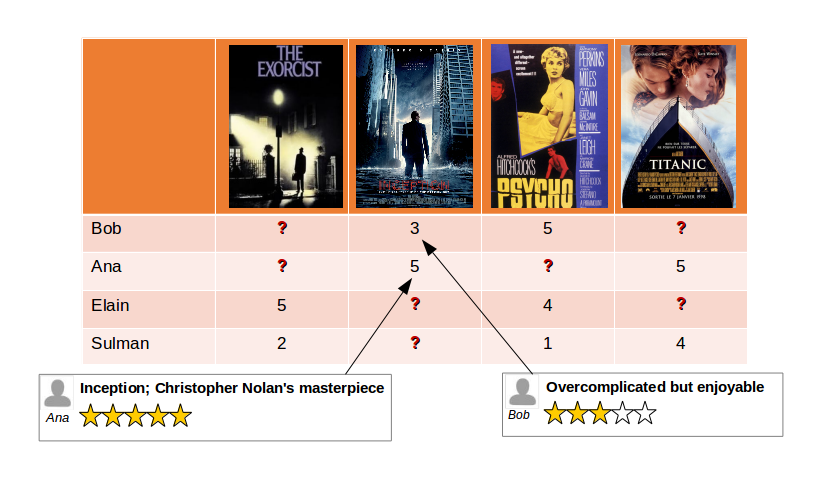
\includegraphics[scale=0.4]{images/4.png}
	\caption{An Example of Matrix R}
	\label{fig:matrix}
\end{figure}

Matrix Factorization is a classic method to solve this problem.
It aims to find a $K$ dimensional low rank matrix $\mathbf{\hat{R}} \in \mathbb{R}^{N \times M}$
where $\mathbf{\hat{R}} = \mathbf{U} \mathbf{V}^\mathrm{T}$ with
$\mathbf{U} \in \mathbb{R}^{N \times K}$ and $\mathbf{V} \in \mathbb{R}^{M \times K}$
are two matrices of rank $K$ encoding a dense representation of the users and items with

\begin{equation}
\begin{aligned}
	\argmin_{\mathbf{U},\mathbf{V}}
	\sum_{(i,j) \in \mathcal{K}(\mathbf{R})}
	( r_{ij} - \overline{\mathbf{u}}_i^{\mathrm{T}} \overline{\mathbf{v}}_j ) ^ 2 +
	\lambda ( \left\| \overline{\mathbf{u}}_i \right\|_{Fro}^2 +
	\left\| \overline{\mathbf{v}}_j \right\|_{Fro}^2 )
\end{aligned}
\end{equation}

where $\mathcal{K}(\mathbf{R})$ is the set of indices of known ratings,
$\overline{\mathbf{u}}_i$ and $\overline{\mathbf{v}}_j$
are the corresponding line vectors of $\mathbf{U}$ and $\mathbf{V}$,
$\lambda$ is the coefficient that controls the influence of L2 regularization,
and $\left\| \cdot \right\|_{Fro}$ is the Frobenius norm.

Matrix Factorization techniques, as the main thrust behind collaborative filtering,
have been developed for many years and keep to be a hot area in both academia and industry.
But it suffers from the problem of cold-start,
i.e. what recommendations to make when a new user or a new item arrives in the system
with the fact that their have no ratings information.
Meanwhile, when the ratings information is too sparse,
the performance of matrix factorization will decrease rapidly.

Side information, such as the users' profiles and the items' properties,
is a effective resource to remit this problem.
In the next section, we will propose a embedding model
to extract latent side information based on the local interest and global interest.

\subsection{Embedding Model}
Collaborative Filtering aims at estimating the ratings
a user would have given to all other items he never interact with
by using the ratings of all the other users.
The basic assumption of collaborative filtering is that
items liked by the same user would be similar
or users like same items would share similar interest.
However, in real-world situations,
it is not always hold because users' interest may change over
a long time period.
Meanwhile, the interest distribution of a user in a fixed time period
are stable and don't change too much.

To describe the phenomenon that interest changes over time,
we propose the definition of \textbf{local interest} and \textbf{global interest}.

\begin{itemize}
\item \textbf{local interest} reflects the interest distribution of a user
in a short and fixed time period.
\item \textbf{global interest} reflects the interest distribution of a user
in a long time period.
\end{itemize}

And we believe that item in the same local interest (i.e. in the same time period)
of a user have a higher possibility to be similar than
items in different local interest.

\begin{figure*}[htbp]
	\centering
	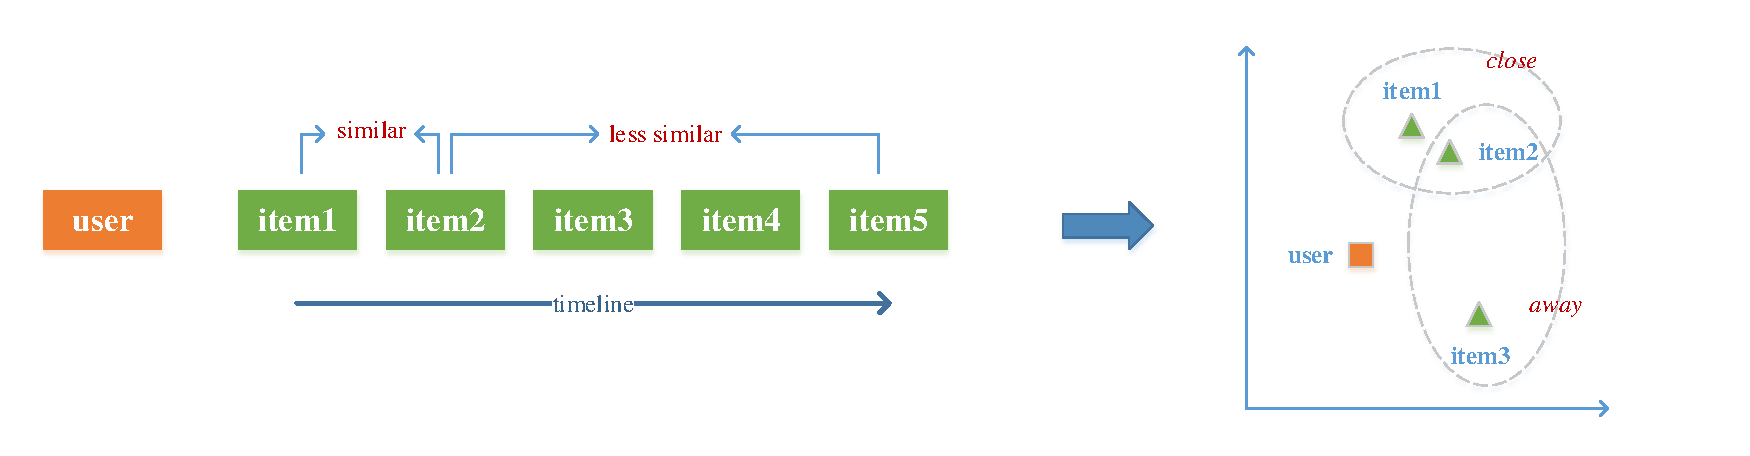
\includegraphics[scale=0.6]{images/1.pdf}
	\caption{A Example for Local Interest and Global Interest}
	\label{fig:example}
\end{figure*}

For example, as illustrated in the left of Figure \ref{fig:example},
given a certain $\mathbf{user}$, we can see he interact with five items
($\mathbf{item1}$ to $\mathbf{item5}$) in the last.
They are list on the time line according to the time order.
Let's assume that the time window size \footnote{We use time window to judge time proximity
instead of extract timestamp here for convenience.} is set to $2$,
Therefore $\mathbf{item1}$ and $\mathbf{item2}$ are in the same local interest,
$\mathbf{item2}$ and $\mathbf{item3}$ are in the same local interest, and so on.
Meanwhile $\mathbf{item2}$ and $\mathbf{item5}$ are in different local interest.
That means $\mathbf{item2}$ has a higher possibility to be similar with $\mathbf{item1}$
than $\mathbf{item5}$.

To describe the similarity preference in mathematical sense,
we project users and items into a low-dimensionality space,
and change the interest similarity into spacial distance.
$\mathbf{item2}$ is close to $\mathbf{item1}$ and far away from $\mathbf{item5}$
in the low-dimensionality space, as shown in the right of Figure \ref{fig:example}.

\begin{figure}[htbp]
	\centering
	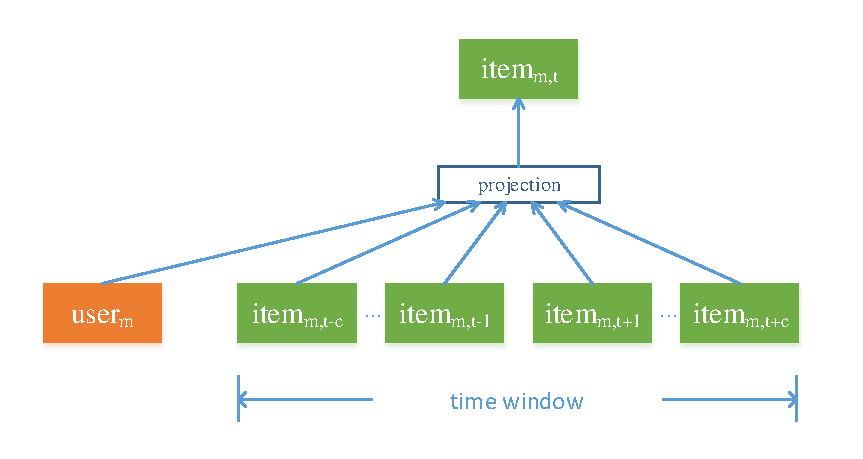
\includegraphics[scale=0.55]{images/2.pdf}
	\caption{Embedding Model for Extracting Interest Similarity from Users and Items}
	\label{fig:embedding}
\end{figure}

Inspired by paragraph2vec algorithm \cite{le2014distributed} for learning
vector representations of words which take advantage of
a word order observed in a sentence,
we choose to use neural network based language model
to embed this interest similarity information.
The embedding model simultaneously learns vector representations of users and items
by considering the user as a global context,
and the architecture of the embedding model is illustrated in Figure \ref{fig:embedding}.

The training data set was derived from users interaction timeline $T$,
which comprises users $u_i (i=1,2,...,N)$ and their interacted items ordered by the interacted time,
$v_{i_1}$, $v_{i_2}$, ..., $v_{i_{L_i}}$,
where $L_i$ denotes number of items interacted by user $u_i$,
which is much less than the amount of items $M$.

More formally, objective of the embedding model is to
maximize the log-likelihood over the set of $T$ of all the interaction timeline,

\begin{equation}
\begin{aligned}
	\sum_{i=1}^{N} \bigg( &p(u_i | v_{i_1}, v_{i_2}, ..., v_{i_{L_n}}) + \\
	                      &\sum_{j=1}^{L_i} p(v_{i_j} | v_{i_{j-c}}, ..., v_{i_{j-1}}, v_{i_{j+1}},..., v_{i_{j+c}}, u_i) \bigg)
\end{aligned}
\end{equation}

where $c$ is the time window size.
$p(u_i | v_{i_1}, v_{i_2}, ..., v_{i_{L_i}})$ is the probability to generate
the global interest of $u_i$ based on all items he interacted.
The prediction task is typically done via a multiclass classifier,
such as softmax. There, we have

\begin{equation}
	p(u_i | v_{i_1}, v_{i_2}, ..., v_{i_{L_i}}) =
	\frac
	{
		exp ( \overline{\mathbf{v}}_{1}^{\mathrm{T}} \mathbf{v}_{u_i}^{'} )
	}
	{
		\sum_{k=1}^{V} exp ( \overline{\mathbf{v}}_{1}^{\mathrm{T}} \mathbf{v}_{k}^{'} )
	}
\end{equation}

where $\mathbf{v}_{u_i}^{'}$ is the output vector representation of $u_i$,
$V$ is the set of the whole items,
and $\overline{\mathbf{v}}_{1}$ is averaged input vector representation of all the items
interacted by user $u_i$, i.e.

\begin{equation}
	\overline{\mathbf{v}}_{1} = \frac{\sum_{j=1}^{T_i} \mathbf{v}_{v_{i_j}}}{T_i}
\end{equation}

$p(v_{i_j} | v_{i_{j-c}}, ..., v_{i_{j-1}}, v_{i_{j+1}},..., v_{i_{j+c}}, u_i)$
is the probability to generate the interest distribution of $v_{i_j}$
based on items in the same local interest and the user's global interest.
Similarly, using softmax multiclass classifier we have

\begin{equation}
	p(v_{i_j} | v_{i_{j-c}}, ..., v_{i_{j-1}}, v_{i_{j+1}},..., v_{i_{j+c}}, u_i) =
	\frac
	{
		exp( \overline{\mathbf{v}}_{2}^{\mathrm{T}} \mathbf{v}_{v_{i_j}}^{'} )
	}
	{
		\sum_{k=1}^{V} exp( \overline{\mathbf{v}}_{2}^{\mathrm{T}} \mathbf{v}_{k}^{'} )
	}
\end{equation}

where $\mathbf{v}_{v_{i_j}}^{'}$ is the output vector representation of $v_{i_j}$,
$V$ is the set of the whole items,
and $\overline{\mathbf{v}}_{2}$ is averaged input vector representation of items
int the same local interest and corresponding global interest $u_i$.

\begin{equation}
	\overline{\mathbf{v}}_{2} = \frac{ \mathbf{v}_{v_{i_{j-c}}} + ... + \mathbf{v}_{v_{i_{j-1}}} + 
	\mathbf{v}_{v_{i_{j+1}}} + ... + \mathbf{v}_{v_{i_{j+c}}} + \mathbf{v}_{u_i} }{2c+1}
\end{equation}


\subsection{Learning Model}
With the help of embedding model, we can obtain
the vector representation of users and items
based on the local interest and global interest.
We use the following notations to describe these representations:

\begin{itemize}
	\item $\tilde{\mathbf{u}}_i$ reflects the interest distribution of the $u_i$
	\item $\tilde{\mathbf{v}}_j$ reflects the interest distribution of the $v_j$
	\item $D$ is the length of those representation
\end{itemize}

There are two kinds of side information in collaborative filtering:
users' profiles and items' properties.
Various kinds of information can be used to model these factors.
In some sense, the representation of users and items from the embedding model
could be treat as a kind of side information,
because it distinguish the similarity and difference between users and items,
just like other side information does.
But it doesn't reflect a actual meaning, so we call it the \textbf{latent side information}. 

Inspired by svdfeature algorithm \cite{chen2012svdfeature}, we utilize the feature-based
collaborative filtering to take advantage of the latent side information.
First, we generate the user feature $\alpha_{i}$ and the item feature $\beta_{j}$
for user $u_i$ and item $v_j$.

\begin{equation}
\alpha_{i} = \{ OneHot(u_i), \tilde{\mathbf{u}}_i \}
\end{equation}
\begin{equation}
\beta_{j} = \{OneHot(v_j), \tilde{\mathbf{v}}_j \}
\end{equation}

where $OneHot(u_i)$ is the one hot representation of $u_i$
and $OneHot(v_j)$ is the one hot representation of $v_j$.

Then we predict the rating for $u_i$ and $v_j$

\begin{equation}
\hat{r} = \sum_{i=1}^{n} \alpha_{i} b_{i}^{(u)} + \sum_{i=1}^{m} \alpha_{i} b_{i}^{(i)} +
\left( \sum_{i=1}^{n} \alpha_{i} \textbf{p}_{i} \right) ^ \mathrm{T}
\left( \sum_{i=1}^{m} \beta_{i} \textbf{q}_{i} \right)
\end{equation}

where $\textbf{p}_{i} \in \mathbb{R}^d$ and $\textbf{q}_{i} \in \mathbb{R}^d$
are $d$ dimensional latent factors associated with each feature.
$b_{i}^{(u)}$ and $b_{i}^{(i)}$ are bias parameters that directly influence the prediction.


\section{Experiment}

\subsection{Baseline Models}
We use two popular techniques that are widely used
in both academia and industry as our baseline models.

\textbf{LibMF} is an open source tool
for approximating an incomplete matrix using the product of
two matrices in a latent space.
It provides solvers for real-valued matrix factorization,
binary matrix factorization, and one-class matrix factorization.
It also supports parallel computation in a multi-core machine
using CPU instructions (e.g., SSE) to accelerate vector operations.
Its paper \cite{chin2015fast} won the best paper award
in RecSys 2013.

Factorization machines (FM) are a generic approach that
allows to mimic most factorization models by feature engineering.
This way, factorization machines combine the generality of
feature engineering with the superiority of factorization models
in estimating interactions between categorical variables of large domain.
\textbf{LibFM} \cite{rendle2012factorization} is a software implementation
for factorization machines that features
Stochastic Gradient Descent (SGD) and
Alternating Least Squares (ALS) optimization as well as
Bayesian inference using Markov Chain Monte Carlo (MCMC).
We select ALS optimization in our baseline experiments.

\subsection{Dataset}
We conduct experiments on three benchmark datasets MovieLens-1M, MovieLens-10M and MovieLens-20M
\footnote{http://grouplens.org/datasets/movielens/},
which are commonly used for evaluating collaborative filtering algorithms.
The MovieLens-1M dataset consists of about 1 million ratings of 6040 users and 3706 movies,
and each rating is an integer between 1 (worst) and 5 (best).
The MovieLens-10M dataset consisits of about 10 million ratings of 69878 users and 10677 movies,
the MovieLens-20M dataset consisits of about 20 million ratings of 138493 users and 26744 movies,
and each rating ranges from 0.5 (worst) to 5.0 (best) step by 0.5.
The ratings are highly sparse.
Table \ref{tab:statistics} summarizes the statistics of three datasets.

\begin{table}[htpb]
	\centering
	\caption{Statistics of three datasets}
	\label{tab:statistics}
	\begin{tabular}{|l|c|c|c|c|}
		\hline
		\textbf{Dataset} & \textbf{\#Users} & \textbf{\#Items} & \textbf{\#Ratings} & \textbf{Sparsity} \\
		\hline
		ML-1M  & 6,040   & 3,706  & 1,000,209  & 95.53\% \\
		ML-10M & 69,878  & 10,677 & 10,000,054 & 98.66\% \\
		ML-20M & 138,493 & 26,744 & 20,000,263 & 99.46\% \\
		\hline
	\end{tabular}
\end{table}

\subsection{Metrics}
We employ the root mean squared error (RMSE) and mean absolute error (MAE) as the evaluation metric.
RMSE and MAE are defined as:
\begin{equation}
	RSME = \sqrt{ \frac{1}{N} \sum_{i,j} I_{ij} (R_{ij} - \hat{R}_{ij})^2 }
\end{equation}
\begin{equation}
	MAE = \frac{1}{N} \sum_{i,j} I_{ij} |R_{ij} - \hat{R}_{ij}|
\end{equation}
where $N$ is the total number of ratings in the test set,
$R_{ij}$ is the ground-truth rating of user $i$ for item $j$,
$\hat{R_{ij}}$ denotes the corresponding predicted rating,
and $I_{ij}$ is abinary matrix that indicates the ratings in the test set.




\begin{table*}[htpb]
	\centering
	\caption{MSRE}
	\label{tab:msre}
	\begin{tabular}{|l|c|c|c|c|}
		\hline
		\textbf{Algorithms} & \textbf{MovieLens-1M} & \textbf{MovieLens-10M} & \textbf{MovieLens-20M} \\
		\hline
		LibMF & 0.8526 $\pm$ 2.4e-3 & 0.8526 $\pm$ 2.4e-3 & 0.8526 $\pm$ 2.4e-3 \\
		LibFM & 0.8526 $\pm$ 2.4e-3 & 0.8526 $\pm$ 2.4e-3 & 0.8526 $\pm$ 2.4e-3 \\
		LTM   & 0.8526 $\pm$ 2.4e-3 & 0.8526 $\pm$ 2.4e-3 & 0.8526 $\pm$ 2.4e-3 \\
		\hline
	\end{tabular}
\end{table*}


\section{Conclusions}


\section{Acknowledgments}
The work reported in this paper is supported by the National Natural Science Foundation of China Grant 61370116.
We thank anonymous reviewers for their beneficial comments.
We also thank Feifan Fan and Yue Fei for valuable suggestions related to this paper.

\bibliographystyle{abbrv}
\bibliography{sigproc}

\end{document}
